\documentclass[conference]{IEEEtran}
\IEEEoverridecommandlockouts
% The preceding line is only needed to identify funding in the first footnote. If that is unneeded, please comment it out.
\usepackage{cite}
\usepackage{amsmath,amssymb,amsfonts}
\usepackage{algorithmic}
\usepackage{graphicx}
\usepackage{textcomp}
\usepackage{xcolor}

\usepackage{multirow}


\def\BibTeX{{\rm B\kern-.05em{\sc i\kern-.025em b}\kern-.08em
    T\kern-.1667em\lower.7ex\hbox{E}\kern-.125emX}}
\begin{document}

\title{Pattern-based monte carlo simulation for AMR electricty load analysis\\
% {\footnotesize \textsuperscript{*}Note: Sub-titles are not captured in Xplore and
% should not be used}
\thanks{PEA, AIT, NEU}
}

\author{\IEEEauthorblockN{1\textsuperscript{st} Pornchai Chaweewat}
\IEEEauthorblockA{\textit{EECC} \\
\textit{AIT)}\\
Pathumthani, Thailand \\
chaweewat.p@gmail.com}
\and
\IEEEauthorblockN{2\textsuperscript{nd} Weerakorn Ongsakul}
\IEEEauthorblockA{\textit{EECC} \\
\textit{AIT)}\\
Pathumthani, Thailand \\
email address}
\and
\IEEEauthorblockN{3\textsuperscript{rd} Jai Govind Singh}
\IEEEauthorblockA{\textit{EECC} \\
\textit{AIT)}\\
Pathumthani, Thailand \\
email address}
\and
\IEEEauthorblockN{4\textsuperscript{th} Ali abur}
\IEEEauthorblockA{\textit{EEC} \\
\textit{NEU}\\
Boston, MA, USA \\
email address}
}

\maketitle

\begin{abstract}
% This document is a model and instructions for \LaTeX.
% This and the IEEEtran.cls file define the components of your paper [title, text, heads, etc.]. *CRITICAL: Do Not Use Symbols, Special Characters, Footnotes,
% or Math in Paper Title or Abstract.
This paper proposes customer behavior analysis for pattern analysis of AMR electricity customer.

In this paper univaraite models for short-term load forecasting based on customer's pattern behavior analysis and probabilistic monte carlo simulation are proposed.
The proposed method were compared with that of other models based on ARIMA, exponential smoothing and neural networks.
Application examples confirm valuable properties of the proposed approaches and their high accuracy.
\end{abstract}

\begin{IEEEkeywords}
Autometic meter reading, confidence interval
\end{IEEEkeywords}

\section{Introduction}
Here is introduction.
In a revolutionary change in enegy section transform the traditional unidirectional electricty grid replaced by bidirectional or smart grid (SG).
As a results of increasing in number of Intelligent Electronic Devices (IEDs) in the power system, especailly metering field.
Consequently, there are repidly jump in enormous data volume in power system for storage, mining, sharing and visualization\cite{b1}.
The advance meter read (AMR) with 15-min read intervals has also been develop to replacve the traditional managtic once a month reading meters.
The AMR reads 96 data per day and carries out 2880 data per month, which means that 2880 times customer data are fed to utility.
In addition, other states variables also transported.
%why data is importation to Smartgrid, utility

% why amr is need?

% why need to analysis pattern
In previous work, there is observation that the forecasting accuracy highly depend on hourly load patterns incorporate with other variables\cite{b2}. In addition, it can also help in long term applications i.e., model customer behavior under various incentive and pricing structures, planning processes\cite{b4}. The behavior of applicace in resident customer helps to forecast shorterm load\cite{b6}.


% why monte carlo simulation
% Monte Carlo simulation is a computerized mathematical technique that allows people to account for risk in quantitative analysis and decision making. The technique is used by professionals in such widely disparate fields as finance, project management, energy, manufacturing, engineering, research and development, insurance, oil & gas, transportation, and the environment.
%
% Monte Carlo simulation furnishes the decision-maker with a range of possible outcomes and the probabilities they will occur for any choice of action.. It shows the extreme possibilities—the outcomes of going for broke and for the most conservative decision—along with all possible consequences for middle-of-the-road decisions.
%
% The technique was first used by scientists working on the atom bomb; it was named for Monte Carlo, the Monaco resort town renowned for its casinos. Since its introduction in World War II, Monte Carlo simulation has been used to model a variety of physical and conceptual systems.


%contribution
In this article, we propose to generate behavior pattern for AMR customer consumption using confidence interval and Monte Carlo simulation. In particular, we make the following contributions:
\begin{itemize}
  \item We show how to extrat a feature of customer consumption behavior by confidence interval with quantile values in order to reduce mumber of data.
  \item We formulate probabilistic function of individual customer behavior from extracted features.
  \item We deploy Monte Carlo simulation technique to simulate power consumption using individual probabilistic customer behavior.
\end{itemize}


\section{Literature reviews}
Here is Literature reviews.

%what we has use AMR data
The AMR data and individual major applicance usage learning are used to predict short-term residential load using Long short-term memory (LSTM) technique\cite{b6}.

The big data has brought numberous tengible benefits to utilities and electricity uesers, which can be systemically concluded as follows:

\begin{itemize}
  \item \textit{Increasing System Stability & Reliability:} Wide area mornitoring require numberous of measurement units, especailly phase measurement units (PMUs) to ensure that the operator can manage system stability. In coorporate with AMR or Smart meter could help in this situation[cite ????].
  \item \textit{Increasing Asset Utilization & Efficiency:} With low accuray of GIS input data, the distribution network topology need to be verified, especially the under ground feeder which are difficult to check\cite{b8}. The big data proces could help to develop modeling of secondary size of transformer as well as energy theft\cite{b7}.
  \item \textit{Better Customer Experience & Satisfaction:} Demand response program is an effective way to manage power balance during high congestion period as well as high tariff. The customer who engaging though demand response program could reduce their energy bill or earn incentives [cite ???].
\end{itemize}

There is several benefits of deploying AMR at homes and office. The mass rollout enables easier billing, fraud detection, forewarning of blackouts, smart real-time pricing schemes, demand response and efficient energy utilization.
However, to acheive aboved benefits, there need advanced data analytics, especailly customer behavior analysis, which is the main motivation of this study.

In addition, the customer pattern also was clustered using Markov model with CFSFDP\cite{b5}
%which method was used to formulate customer pattern
In previous works, electrical customer consumption's pattern is formulated using various approach. Gaussian mixture model (GMM) is proposed to formaulate individual AMR-based electricity comsumption pattern\cite{b3}.

So far, there is less number of article study on electricity customer behavior.
The contribution of this work is ...


\section{Problem Formulation}
Here is Problem formulation.
The overall methodology is shown in Figure\ref{fig.overall_methodology}

\begin{figure}[htbp]
  \centerline{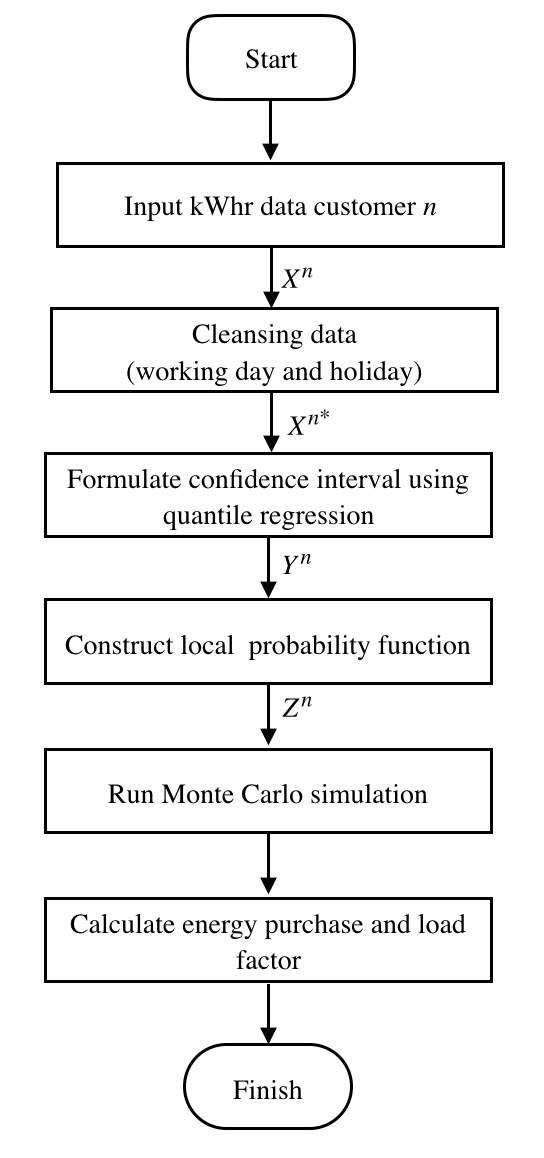
\includegraphics{images/overall_methodology.png}}
  \caption{Conceptual methodology}
  \label{fig.overall_methodology}
\end{figure}



% \subsection{Data collection}
% where the data comes from: PEA
% total number of AMR customer:
% duration: 2 years???
\subsection{Pattern formulation using confidence intervals for quantiles calculation}
In this paper 15 minutes based kilowatt data are collected from AMR system. These data are accumulate into 30-minutes based kiloWatt-hour.

\begin{equation}
X=\big\{ X^{1}, X^{2}, X^{3}, ..., X^{n} \big\}
\label{eq.list_customer}
\end{equation}
\begin{equation}
X^{n}=\big\{ X_{1}^{n}, X_{2}^{n}, X_{3}^{n}, ...,X_{d}^{n},..., X_{366}^{n}\big\}
\label{eq.list_customer_consumption}
\end{equation}
\begin{equation}
X_{d}^{n}=\big\{ X_{d,1}^{n}, X_{d,2}^{n}, X_{d,3}^{n}, ...,X_{d,t}^{n},..., X_{d,48}^{n}\big\}
\label{eq.list_customer_consumption_daily}
\end{equation}
where $X$ is set of customer, $X^{n}$ is set of daily consumtion of custome $n$, $X_{d}^n$ is set of 30 minutes based power consumption (kWhr) of customer $n$ on day $d$. $x_{d,t}^{n}$ is power consumption of customer $n$ on day $d$ at time $t$.
The equation~(\ref{eq.list_customer})-(\ref{eq.list_customer_consumption_daily}) are cleansing into equation~(\ref{eq.list_customer_comsumption_at_t}).
$X^{n*}$ is set of power consumption at individual time step. $X_{t}^{n*}$ is set of power consumption at time $t$ of customer $n$.
\begin{equation}
X^{n*}=\big\{ X_{1}^{n*}, X_{2}^{n*}, X_{3}^{n*}, ..., X_{t}^{n*}, ..., X_{48}^{n*} \big\}
\label{eq.list_customer_comsumption_at_t}
\end{equation}
The $X^{n*}$ is cleansing raw data prepared to feature extraction process. As memntion above, this paper proposed confidential interval at quantile value as extracted feature. The extracted feature processes are shown in equation~(\ref{eq.quantile_of_customer})-~(\ref{eq.quantile_of_customer_at_t}).
\begin{equation}
  Y^{n}=\big\{ Y_{1}^{n}, Y_{2}^{n}, Y_{3}^{n}, ..., Y_{t}^{n}, ..., Y_{48}^{n} \big\}
  \label{eq.quantile_of_customer}
\end{equation}
\begin{equation}
  Y_{t}^{n}=\big\{ Y_{t,0}^{n}, Y_{t,0.05}^{n}, Y_{t,0.1}^{n}, ..., Y_{t,q}^{n}, ..., Y_{t,1}^{n} \big\}
  \label{eq.quantile_of_customer_at_t}
\end{equation}
Where $Y^{n}$ is representing set of extract feature of customer $n$ at individual time period, $Y_{t}^{n}$ is set of extracted feature of customer $n$ at time period $t$ which content 20 step of quantile value, $q$, (0 to 1 at 0.05 step size).
$Y_{t,q}^{n}$ is formulated using equation~(\ref{eq.quantile_formular}).

\begin{equation}
  Y_{t,q}^{n}=\int_{q-1}^{q} F_{X^{n*}}(q) dq
  \label{eq.quantile_formular}
\end{equation}
Where $F_{X^{n*}}$ is commulative distribution function of power consumption of customer $n$ at time $t$. So, $Y_{t,q}^{n}$ is expected power consumption of customer $n$ at time period $t$, and quantile $q$.

Hence, we can extract customer behavior feature as well as reduce number of process data in next step.

\subsection{Continuous Probability Distribution constuction}

\begin{equation}
Z^{n}=\big\{ Z_{0}^{n}, Z_{1}^{n}, Z_{3}^{n}, ..., Z_{t}^{n}, ..., Z_{48}^{n} \big\}
\label{eq.CPD_customer}
\end{equation}
\begin{equation}
Z_{t}^{n}=\big\{ z_{0,50}^{n}, z_{50,100}^{n}, z_{100,150}^{n}, ..., z_{a,b}^{n}, ..., z_{19500,2000}^{n} \big\}
\label{eq.CPD_customer_at_t}
\end{equation}
where $Z^{n}$ is set of continous probability distribution function of power consumption of customer $n$.
$Z_{t}^{n}$ is set of continous probability distribution function of power consumption of customer $n$ at time $t$ with difference consumption range (from 0 to 20,000 kiloWatt-hour with 50 kiloWatt-hour step size).
$z_{a,b}^{n}$ is probability of power consumption between lower $a$ and upper $b$ kiloWatt-hour of customer $n$ which is be formulation by equation~(\ref{eq.cpd_construction}).


\begin{equation}
z_{a,b}^{n}=\text{P}\big[ a \le Y_{t}^{n} \le b \big] = \int_{a}^{b} Y_{t}^{n}dY_{t}^{n}
\label{eq.cpd_construction}
\end{equation}

where $a$ and $b$ is lower and upper kilowatt-hour in range $\big[ a,b \big]$.

\subsection{Monte carlo simulation}

From $Z^{n}$, monte carlo simulation generate electricity consumption as

\begin{equation}
P^{n}=\big\{ P_{1}^{n}, P_{2}^{n}, P_{3}^{n}, ..., P_{i}^{n}, ..., P_{m}^{n}\big\}
\label{eq.generated_kW_cust_n}
\end{equation}
\begin{equation}
P_{i}^{n}=\big\{ P_{i,1}^{n}, P_{i,2}^{n}, P_{i,3}^{n}, ..., P_{i,t}^{n}, ..., P_{i,48}^{n}\big\}
\label{eq.generated_kW_cust_n_at_sample_i}
\end{equation}

where $m$ is number of samples. $P_{i,t}^{n}$ is generated electricity consumption of customer $n$ at time $t$ at sample $i$.


\subsection{Find cost and load factor}


\begin{equation}
C_{i}^{n}=\sum_{t=1}^{48}   P_{i,t}^{n} \times a_{t}
\label{eq.cost}
\end{equation}

where $C_{i}^{n}$ is cost of energy purchasing of customer $n$ at sample $i$, $a_{t}$ is electricity tariff at time $t$.

\begin{equation}
\text{LF}_{i}^{n}=\frac{\text{average}(P_{i}^{n})}{\text{max}(P_{i}^{n})}
\label{eq.load_factor}
\end{equation}

where $\text{LF}_{i}^{n}$ is load factor of customer $n$ at sample $i$.

\section{Test Cases and Results}
In this study, AMR data is collected from PEA. This dataset comprehensively records the quarter hourly kilowatt reading of 35 commercial and industrial customers. We accomulate the kilowatt reading into kilowatt hour for every 30 minutes. The AMR customer names are change to alias for information security.

In feature extraction processes, total number of 70,272 raw data for each individual customer (2 years of collections) can be reduce to 1,920 data points (960 point for each working day and holiday).


The result of MC simulation with numbers of samples (20 samples) are consider as witness in this study
Here is results. See in \ref{tab.res_cost_working_day}, \ref{tab.res_LF_working_day}

\begin{table}[]
  \caption{Energy cost per day on workind day}
  \begin{center}
  \begin{tabular}{ccccc}
  \hline
  \multirow{2}{*}{AMR-ID} & \multicolumn{2}{c}{Raw data}               & \multicolumn{2}{c}{Proposed approach (20 samples)}\\
                          & \multicolumn{1}{c}{Mean} & \multicolumn{1}{c}{SD} & \multicolumn{1}{c}{mean}  & \multicolumn{1}{c}{sd} \\
  \hline
  21652 & 75,139 & 14,264 & 75,502 & 11,558 \\
136898 & 153,630 & 23,736 & 152,176 & 12,202 \\
137091 & 34,053 & 9,608 & 37,134 & 3,980 \\
137138 & 33,384 & 16,728 & 34,907 & 3,805 \\
42432 & 236,816 & 44,446 & 238,527 & 11,596 \\
66543 & 12,456 & 2,569 & 13,103 & 988 \\
21654 & 6,795 & 6,970 & 9,151 & 1,781 \\
42421 & 67,473 & 11,738 & 65,978 & 4,034 \\
42423 & 5,743 & 3,470 & 6,245 & 2,119 \\
43958 & 70,504 & 16,975 & 71,375 & 6,810 \\
137110 & 11,973 & 2,166 & 13,418 & 951 \\
21655 & 5,579 & 1,591 & 5,730 & 397 \\
42431 & 12,357 & 3,402 & 11,882 & 975 \\
44834 & 63,665 & 11,412 & 64,856 & 2,979 \\
56452 & 213,943 & 35,413 & 215,219 & 9,267 \\
56457 & 36,415 & 4,492 & 36,151 & 1,431 \\
56458 & 28,128 & 3,577 & 27,797 & 1,401 \\
124642 & 65,564 & 9,881 & 64,834 & 2,205 \\
124647 & 56,148 & 8,723 & 55,809 & 1,814 \\
124649 & 241,325 & 39,482 & 238,368 & 10,597 \\
124656 & 57,745 & 7,114 & 57,947 & 2,554 \\
124683 & 15,237 & 2,342 & 15,043 & 750 \\
185767 & 22,119 & 5,746 & 22,564 & 1,361 \\
56448 & 51,399 & 8,024 & 50,880 & 2,564 \\
136900 & 84,763 & 4,738 & 84,603 & 2,969 \\
137094 & 237,926 & 33,501 & 236,738 & 14,264 \\
164978 & 11,111 & 3,533 & 11,625 & 1,055 \\
189318 & 147,381 & 18,182 & 148,718 & 4,839 \\
193781 & 59,164 & 37,639 & 61,509 & 6,127 \\
44318 & 31,611 & 8,814 & 31,667 & 2,099 \\
124687 & 4,702 & 725 & 5,637 & 300 \\
21689 & 62,114 & 12,386 & 62,917 & 6,148 \\
44831 & 57,599 & 8,382 & 58,446 & 1,941 \\
56459 & 11,456 & 5,235 & 11,453 & 1,353 \\
124678 & 56,828 & 28,156 & 57,598 & 5,405 \\
  \hline
  \end{tabular}
  \label{tab.res_cost_working_day}
  \end{center}
\end{table}

\begin{table}[]
  \caption{LF per day on workind day}
  \begin{center}
  \begin{tabular}{ccccc}
  \hline
  \multirow{2}{*}{AMR-ID} & \multicolumn{2}{c}{Raw data}               & \multicolumn{2}{c}{Proposed approach (20 samples)}\\
                          & \multicolumn{1}{c}{Mean} & \multicolumn{1}{c}{SD} & \multicolumn{1}{c}{mean}  & \multicolumn{1}{c}{sd} \\
  \hline

  21652 & 0.458 & 0.078 & 0.422 & 0.076 \\
136898 & 0.595 & 0.080 & 0.422 & 0.063 \\
137091 & 0.403 & 0.098 & 0.256 & 0.040 \\
137138 & 0.459 & 0.084 & 0.312 & 0.042 \\
42432 & 0.551 & 0.057 & 0.428 & 0.039 \\
66543 & 0.396 & 0.051 & 0.326 & 0.041 \\
21654 & 0.332 & 0.110 & 0.209 & 0.036 \\
42421 & 0.455 & 0.046 & 0.369 & 0.037 \\
42423 & 0.227 & 0.111 & 0.114 & 0.048 \\
43958 & 0.753 & 0.175 & 0.720 & 0.070 \\
137110 & 0.523 & 0.080 & 0.401 & 0.087 \\
21655 & 0.408 & 0.091 & 0.272 & 0.051 \\
42431 & 0.482 & 0.090 & 0.320 & 0.044 \\
44834 & 0.569 & 0.090 & 0.524 & 0.053 \\
56452 & 0.620 & 0.089 & 0.554 & 0.048 \\
56457 & 0.567 & 0.060 & 0.498 & 0.031 \\
56458 & 0.621 & 0.083 & 0.570 & 0.057 \\
124642 & 0.583 & 0.059 & 0.528 & 0.046 \\
124647 & 0.543 & 0.063 & 0.480 & 0.044 \\
124649 & 0.655 & 0.061 & 0.523 & 0.048 \\
124656 & 0.592 & 0.082 & 0.495 & 0.080 \\
124683 & 0.520 & 0.071 & 0.431 & 0.053 \\
185767 & 0.561 & 0.089 & 0.412 & 0.057 \\
56448 & 0.571 & 0.051 & 0.507 & 0.065 \\
136900 & 0.710 & 0.056 & 0.663 & 0.060 \\
137094 & 0.350 & 0.035 & 0.310 & 0.028 \\
164978 & 0.464 & 0.111 & 0.314 & 0.053 \\
189318 & 0.682 & 0.050 & 0.582 & 0.050 \\
193781 & nan & nan & 0.350 & 0.082 \\
44318 & 0.613 & 0.073 & 0.469 & 0.057 \\
124687 & 0.553 & 0.047 & 0.522 & 0.048 \\
21689 & 0.232 & 0.030 & 0.221 & 0.021 \\
44831 & 0.533 & 0.060 & 0.463 & 0.059 \\
56459 & 0.366 & 0.078 & 0.257 & 0.057 \\
124678 & 0.673 & 0.094 & 0.407 & 0.035 \\
  \hline
  \end{tabular}
  \label{tab.res_LF_working_day}
  \end{center}
\end{table}


\section{Conclusion}
Here is Conclusion.

The major contribution of this work is to propose new simulation univariate monte carlo simulation models based on pattern of customer behavior analysis.


\section*{Acknowledgment}
I am vary grateful to Mr. Pradya Panyainkeaw, AMR division, PEA, Thailand for supplying data, and AIT, PEA for financial support.


\section*{References}

\begin{thebibliography}{00}
\bibitem{b1} Depuru SSSR, Wang L, Devabhaktuni V. Smart meters for power grid: challenges, issues, advantages and status. Renew Sustain Energy Rev 2011;15(6):2736–42.
\bibitem{b2} Srinivasan D. Evolving artificial neural networks for short term load forecasting. Neurocomputing 1998;23:265–76.1534.
\bibitem{b3} Chaweewat P., Singh J. G. , Ongsakul W. A Two Stages Pattern Recognition for Time-of-use Customers based on Behavior Analytic by Using Gaussian Mixture Models and K-mean Clustering: a Case Study of PEA, Thailand, 2018 International Conference and Utility Exhibition on Green Energy for Sustainable Development (ICUE)
\bibitem{b4} N. Yu, S. Shah, R. Johnson, R. Sherick, M. Hong, and K. Loparo, “Big data analytics in power distribution systems,” 2015 IEEE Power Energy Soc. Innov. Smart Grid Technol. Conf., pp. 1–5, 2015.
\bibitem{b5} Y. Wang, Q. Chen, C. Kang, and Q. Xia, “Clustering of Electricity Consumption Behavior Dynamics Toward Big Data Applications,” IEEE Trans. Smart Grid, vol. 7, no. 5, pp. 2437–2447, 2016
\bibitem{b6} W. Kong, Z. Y. Dong, D. J. Hill, F. Luo and Y. Xu, "Short-Term Residential Load Forecasting Based on Resident Behaviour Learning," in IEEE Transactions on Power Systems, vol. 33, no. 1, pp. 1087-1088, Jan. 2018.
\bibitem{b7} Jokar P, Arianpoo N, Leung VCM. Electricity theft detection in AMI using customers' consumption patterns. IEEE Trans Smart Grid 2016;7(1):216–26.
\bibitem{b8} Luan W, Peng J, Maras M, et al. Smart meter data analytics for distribution network connectivity verification. IEEE Trans Smart Grid 2015;6(4), [1–1].
\end{thebibliography}


% \section{Introduction}
% This document is a model and instructions for \LaTeX.
% Please observe the conference page limits.
%
% \section{Ease of Use}
%
% \subsection{Maintaining the Integrity of the Specifications}
%
% The IEEEtran class file is used to format your paper and style the text. All margins,
% column widths, line spaces, and text fonts are prescribed; please do not
% alter them. You may note peculiarities. For example, the head margin
% measures proportionately more than is customary. This measurement
% and others are deliberate, using specifications that anticipate your paper
% as one part of the entire proceedings, and not as an independent document.
% Please do not revise any of the current designations.
%
% \section{Prepare Your Paper Before Styling}
% Before you begin to format your paper, first write and save the content as a
% separate text file. Complete all content and organizational editing before
% formatting. Please note sections \ref{AA}--\ref{SCM} below for more information on
% proofreading, spelling and grammar.
%
% Keep your text and graphic files separate until after the text has been
% formatted and styled. Do not number text heads---{\LaTeX} will do that
% for you.
%
% \subsection{Abbreviations and Acronyms}\label{AA}
% Define abbreviations and acronyms the first time they are used in the text,
% even after they have been defined in the abstract. Abbreviations such as
% IEEE, SI, MKS, CGS, ac, dc, and rms do not have to be defined. Do not use
% abbreviations in the title or heads unless they are unavoidable.
%
% \subsection{Units}
% \begin{itemize}
% \item Use either SI (MKS) or CGS as primary units. (SI units are encouraged.) English units may be used as secondary units (in parentheses). An exception would be the use of English units as identifiers in trade, such as ``3.5-inch disk drive''.
% \item Avoid combining SI and CGS units, such as current in amperes and magnetic field in oersteds. This often leads to confusion because equations do not balance dimensionally. If you must use mixed units, clearly state the units for each quantity that you use in an equation.
% \item Do not mix complete spellings and abbreviations of units: ``Wb/m\textsuperscript{2}'' or ``webers per square meter'', not ``webers/m\textsuperscript{2}''. Spell out units when they appear in text: ``. . . a few henries'', not ``. . . a few H''.
% \item Use a zero before decimal points: ``0.25'', not ``.25''. Use ``cm\textsuperscript{3}'', not ``cc''.)
% \end{itemize}
%
% \subsection{Equations}
% Number equations consecutively. To make your
% equations more compact, you may use the solidus (~/~), the exp function, or
% appropriate exponents. Italicize Roman symbols for quantities and variables,
% but not Greek symbols. Use a long dash rather than a hyphen for a minus
% sign. Punctuate equations with commas or periods when they are part of a
% sentence, as in:
% \begin{equation}
% a+b=\gamma\label{eq}
% \end{equation}
%
% Be sure that the
% symbols in your equation have been defined before or immediately following
% the equation. Use ``\eqref{eq}'', not ``Eq.~\eqref{eq}'' or ``equation \eqref{eq}'', except at
% the beginning of a sentence: ``Equation \eqref{eq} is . . .''
%
% \subsection{\LaTeX-Specific Advice}
%
% Please use ``soft'' (e.g., \verb|\eqref{Eq}|) cross references instead
% of ``hard'' references (e.g., \verb|(1)|). That will make it possible
% to combine sections, add equations, or change the order of figures or
% citations without having to go through the file line by line.
%
% Please don't use the \verb|{eqnarray}| equation environment. Use
% \verb|{align}| or \verb|{IEEEeqnarray}| instead. The \verb|{eqnarray}|
% environment leaves unsightly spaces around relation symbols.
%
% Please note that the \verb|{subequations}| environment in {\LaTeX}
% will increment the main equation counter even when there are no
% equation numbers displayed. If you forget that, you might write an
% article in which the equation numbers skip from (17) to (20), causing
% the copy editors to wonder if you've discovered a new method of
% counting.
%
% {\BibTeX} does not work by magic. It doesn't get the bibliographic
% data from thin air but from .bib files. If you use {\BibTeX} to produce a
% bibliography you must send the .bib files.
%
% {\LaTeX} can't read your mind. If you assign the same label to a
% subsubsection and a table, you might find that Table I has been cross
% referenced as Table IV-B3.
%
% {\LaTeX} does not have precognitive abilities. If you put a
% \verb|\label| command before the command that updates the counter it's
% supposed to be using, the label will pick up the last counter to be
% cross referenced instead. In particular, a \verb|\label| command
% should not go before the caption of a figure or a table.
%
% Do not use \verb|\nonumber| inside the \verb|{array}| environment. It
% will not stop equation numbers inside \verb|{array}| (there won't be
% any anyway) and it might stop a wanted equation number in the
% surrounding equation.
%
% \subsection{Some Common Mistakes}\label{SCM}
% \begin{itemize}
% \item The word ``data'' is plural, not singular.
% \item The subscript for the permeability of vacuum $\mu_{0}$, and other common scientific constants, is zero with subscript formatting, not a lowercase letter ``o''.
% \item In American English, commas, semicolons, periods, question and exclamation marks are located within quotation marks only when a complete thought or name is cited, such as a title or full quotation. When quotation marks are used, instead of a bold or italic typeface, to highlight a word or phrase, punctuation should appear outside of the quotation marks. A parenthetical phrase or statement at the end of a sentence is punctuated outside of the closing parenthesis (like this). (A parenthetical sentence is punctuated within the parentheses.)
% \item A graph within a graph is an ``inset'', not an ``insert''. The word alternatively is preferred to the word ``alternately'' (unless you really mean something that alternates).
% \item Do not use the word ``essentially'' to mean ``approximately'' or ``effectively''.
% \item In your paper title, if the words ``that uses'' can accurately replace the word ``using'', capitalize the ``u''; if not, keep using lower-cased.
% \item Be aware of the different meanings of the homophones ``affect'' and ``effect'', ``complement'' and ``compliment'', ``discreet'' and ``discrete'', ``principal'' and ``principle''.
% \item Do not confuse ``imply'' and ``infer''.
% \item The prefix ``non'' is not a word; it should be joined to the word it modifies, usually without a hyphen.
% \item There is no period after the ``et'' in the Latin abbreviation ``et al.''.
% \item The abbreviation ``i.e.'' means ``that is'', and the abbreviation ``e.g.'' means ``for example''.
% \end{itemize}
% An excellent style manual for science writers is \cite{b7}.
%
% \subsection{Authors and Affiliations}
% \textbf{The class file is designed for, but not limited to, six authors.} A
% minimum of one author is required for all conference articles. Author names
% should be listed starting from left to right and then moving down to the
% next line. This is the author sequence that will be used in future citations
% and by indexing services. Names should not be listed in columns nor group by
% affiliation. Please keep your affiliations as succinct as possible (for
% example, do not differentiate among departments of the same organization).
%
% \subsection{Identify the Headings}
% Headings, or heads, are organizational devices that guide the reader through
% your paper. There are two types: component heads and text heads.
%
% Component heads identify the different components of your paper and are not
% topically subordinate to each other. Examples include Acknowledgments and
% References and, for these, the correct style to use is ``Heading 5''. Use
% ``figure caption'' for your Figure captions, and ``table head'' for your
% table title. Run-in heads, such as ``Abstract'', will require you to apply a
% style (in this case, italic) in addition to the style provided by the drop
% down menu to differentiate the head from the text.
%
% Text heads organize the topics on a relational, hierarchical basis. For
% example, the paper title is the primary text head because all subsequent
% material relates and elaborates on this one topic. If there are two or more
% sub-topics, the next level head (uppercase Roman numerals) should be used
% and, conversely, if there are not at least two sub-topics, then no subheads
% should be introduced.
%
% \subsection{Figures and Tables}
% \paragraph{Positioning Figures and Tables} Place figures and tables at the top and
% bottom of columns. Avoid placing them in the middle of columns. Large
% figures and tables may span across both columns. Figure captions should be
% below the figures; table heads should appear above the tables. Insert
% figures and tables after they are cited in the text. Use the abbreviation
% ``Fig.~\ref{fig}'', even at the beginning of a sentence.
%
% \begin{table}[htbp]
% \caption{Table Type Styles}
% \begin{center}
% \begin{tabular}{|c|c|c|c|}
% \hline
% \textbf{Table}&\multicolumn{3}{|c|}{\textbf{Table Column Head}} \\
% \cline{2-4}
% \textbf{Head} & \textbf{\textit{Table column subhead}}& \textbf{\textit{Subhead}}& \textbf{\textit{Subhead}} \\
% \hline
% copy& More table copy$^{\mathrm{a}}$& &  \\
% \hline
% \multicolumn{4}{l}{$^{\mathrm{a}}$Sample of a Table footnote.}
% \end{tabular}
% \label{tab1}
% \end{center}
% \end{table}
%
% \begin{figure}[htbp]
% \centerline{\includegraphics{fig1.png}}
% \caption{Example of a figure caption.}
% \label{fig}
% \end{figure}
%
% Figure Labels: Use 8 point Times New Roman for Figure labels. Use words
% rather than symbols or abbreviations when writing Figure axis labels to
% avoid confusing the reader. As an example, write the quantity
% ``Magnetization'', or ``Magnetization, M'', not just ``M''. If including
% units in the label, present them within parentheses. Do not label axes only
% with units. In the example, write ``Magnetization (A/m)'' or ``Magnetization
% \{A[m(1)]\}'', not just ``A/m''. Do not label axes with a ratio of
% quantities and units. For example, write ``Temperature (K)'', not
% ``Temperature/K''.
%
% \section*{Acknowledgment}
%
% The preferred spelling of the word ``acknowledgment'' in America is without
% an ``e'' after the ``g''. Avoid the stilted expression ``one of us (R. B.
% G.) thanks $\ldots$''. Instead, try ``R. B. G. thanks$\ldots$''. Put sponsor
% acknowledgments in the unnumbered footnote on the first page.
%
% \section*{References}
%
% Please number citations consecutively within brackets \cite{b1}. The
% sentence punctuation follows the bracket \cite{b2}. Refer simply to the reference
% number, as in \cite{b3}---do not use ``Ref. \cite{b3}'' or ``reference \cite{b3}'' except at
% the beginning of a sentence: ``Reference \cite{b3} was the first $\ldots$''
%
% Number footnotes separately in superscripts. Place the actual footnote at
% the bottom of the column in which it was cited. Do not put footnotes in the
% abstract or reference list. Use letters for table footnotes.
%
% Unless there are six authors or more give all authors' names; do not use
% ``et al.''. Papers that have not been published, even if they have been
% submitted for publication, should be cited as ``unpublished'' \cite{b4}. Papers
% that have been accepted for publication should be cited as ``in press'' \cite{b5}.
% Capitalize only the first word in a paper title, except for proper nouns and
% element symbols.
%
% For papers published in translation journals, please give the English
% citation first, followed by the original foreign-language citation \cite{b6}.
%
% \begin{thebibliography}{00}
% \bibitem{b1} G. Eason, B. Noble, and I. N. Sneddon, ``On certain integrals of Lipschitz-Hankel type involving products of Bessel functions,'' Phil. Trans. Roy. Soc. London, vol. A247, pp. 529--551, April 1955.
% \bibitem{b2} J. Clerk Maxwell, A Treatise on Electricity and Magnetism, 3rd ed., vol. 2. Oxford: Clarendon, 1892, pp.68--73.
% \bibitem{b3} I. S. Jacobs and C. P. Bean, ``Fine particles, thin films and exchange anisotropy,'' in Magnetism, vol. III, G. T. Rado and H. Suhl, Eds. New York: Academic, 1963, pp. 271--350.
% \bibitem{b4} K. Elissa, ``Title of paper if known,'' unpublished.
% \bibitem{b5} R. Nicole, ``Title of paper with only first word capitalized,'' J. Name Stand. Abbrev., in press.
% \bibitem{b6} Y. Yorozu, M. Hirano, K. Oka, and Y. Tagawa, ``Electron spectroscopy studies on magneto-optical media and plastic substrate interface,'' IEEE Transl. J. Magn. Japan, vol. 2, pp. 740--741, August 1987 [Digests 9th Annual Conf. Magnetics Japan, p. 301, 1982].
% \bibitem{b7} M. Young, The Technical Writer's Handbook. Mill Valley, CA: University Science, 1989.
% \end{thebibliography}
% \vspace{12pt}
% \color{red}
% IEEE conference templates contain guidance text for composing and formatting conference papers. Please ensure that all template text is removed from your conference paper prior to submission to the conference. Failure to remove the template text from your paper may result in your paper not being published.

\end{document}
